\section{Connecting The Devices}
In \cref{sec:communication_methods} and \cref{sec:transmit} we decided to use WiFi Direct and Protobufs accordingly.
This section will explain how they inter-operate with our app.
% Vi har valgt wifi direct
% Vi har valgt at bruge protobufs

\subsection{Preparing the App}
We have previous, in \cref{sec:foundation_of_our_android_app}, explained that we utilize a sample music player.
Now we have the desire that not all devices should enter that app on start up, such that we can have a master-slave relation between the devices.

\begin{figure}[ht] 
  \begin{subfigure}[b]{0.5\linewidth}
    \centering
    %\includegraphics[width=0.75\linewidth]{example-image-a} 
    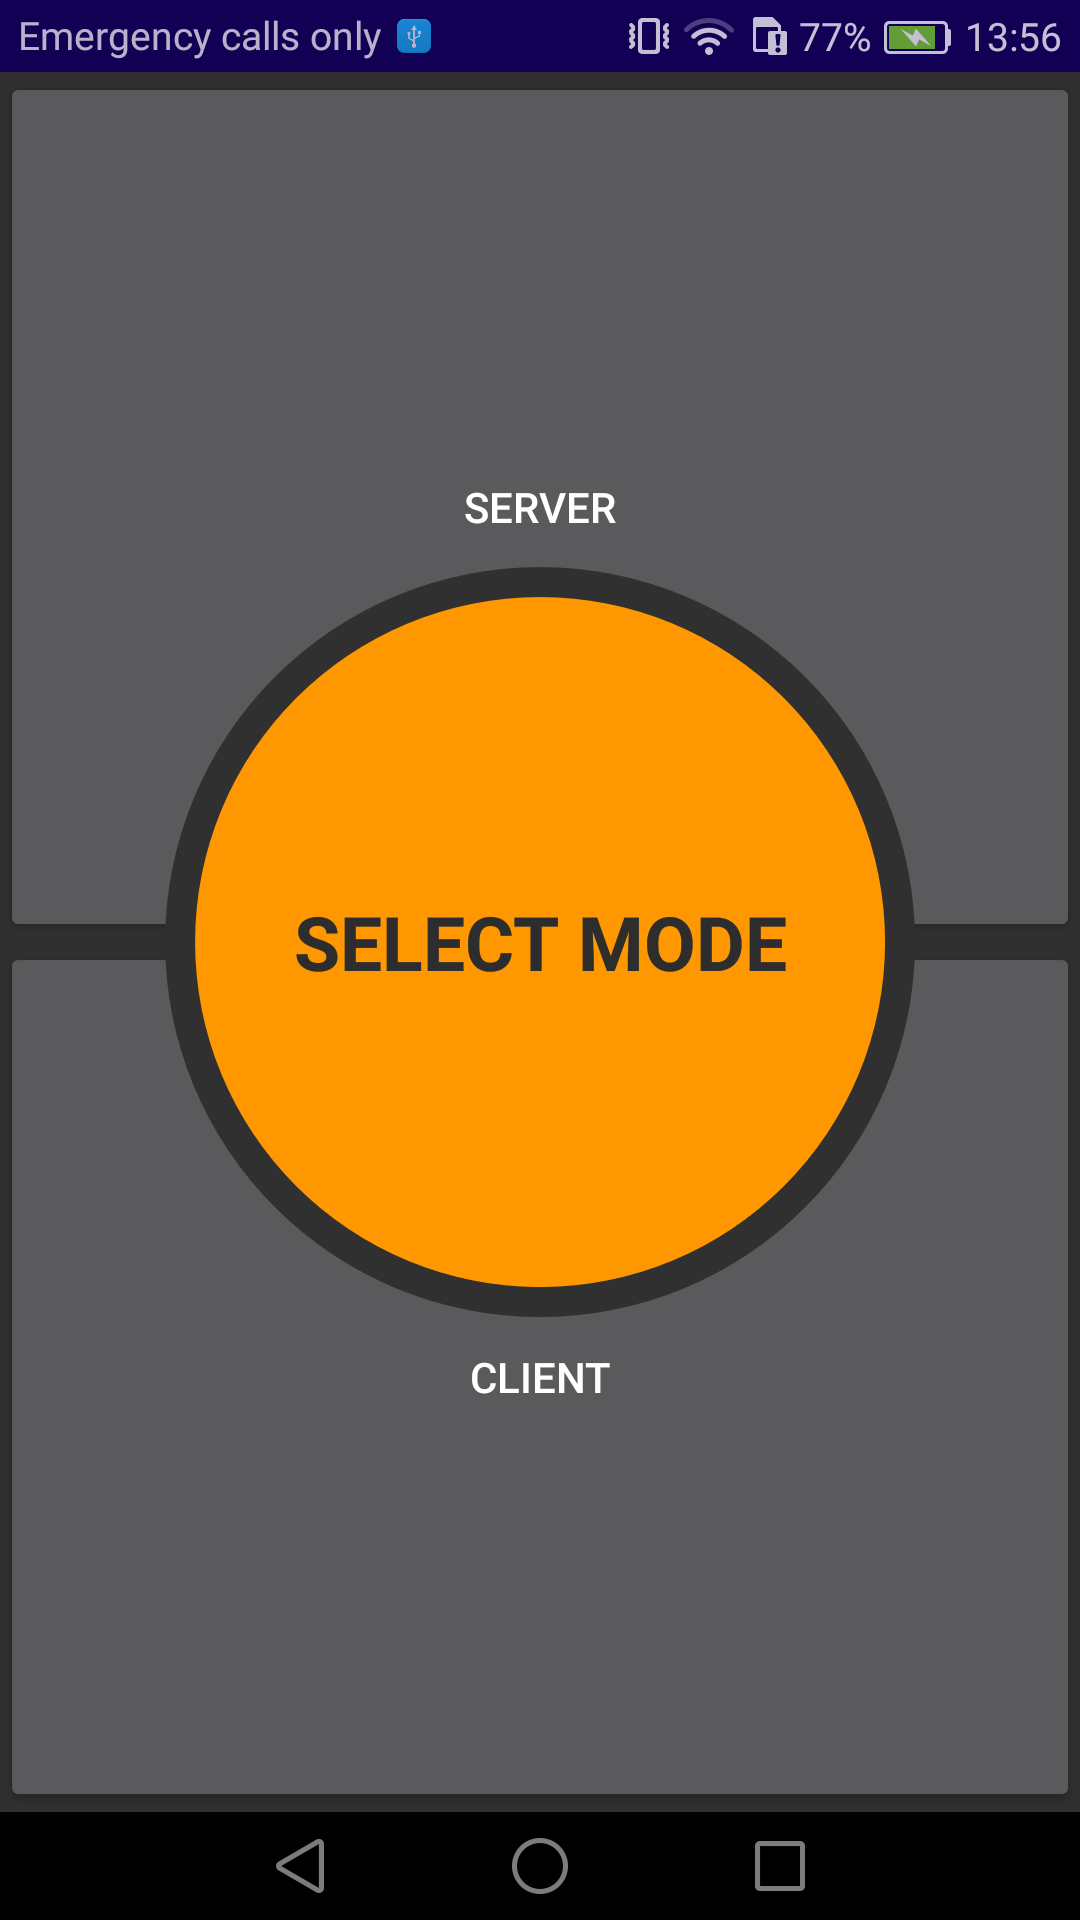
\includegraphics[trim={0cm 0cm 0cm 0cm}, clip, height=10cm]{img/ui/mode_selection.png}
    \caption{Mode Selection} 
    \label{fig:mode_selection} 
    \vspace{4ex}
  \end{subfigure}%% 
  \begin{subfigure}[b]{0.5\linewidth}
    \centering
    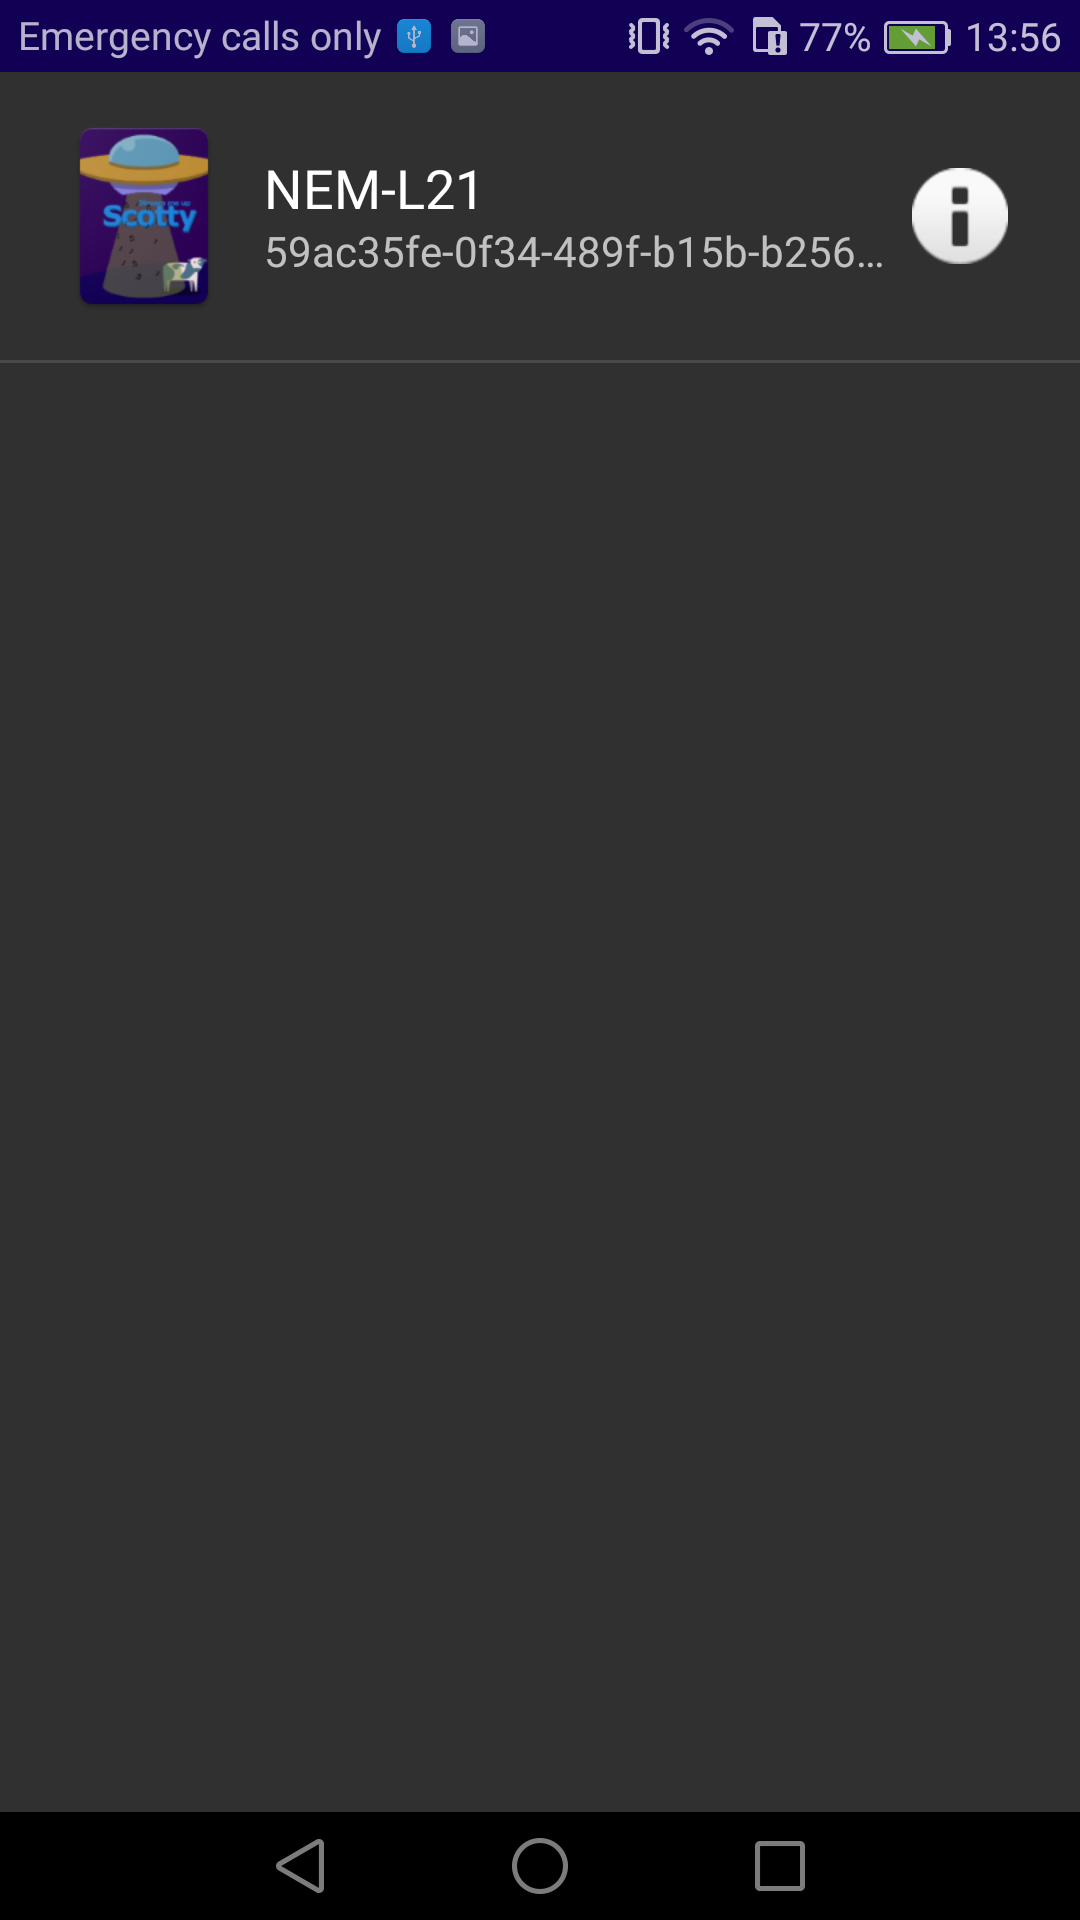
\includegraphics[trim={0cm 0cm 0cm 0cm}, clip, height=10cm]{img/ui/group_selection.png}
    \caption{Group Selection} 
    \label{fig:group_selection} 
    \vspace{4ex}
  \end{subfigure} 
  \caption{The user interface relevant for connecting devices.}
  \label{fig:connecting} 
\end{figure}

\subsection{Service Discovery}

The first problem which must be handled is discovering peers. 


% Service discovery
% Initial connection
% Persistent socket
% Diagram ???
